\documentclass{article}
\usepackage{amsmath}
\usepackage[margin=0.5in]{geometry}
\usepackage{graphicx}
\usepackage{amsmath}
\usepackage{tikz}
\usepackage{xcolor}
\usetikzlibrary{calc}
\usepackage{hyperref}

\begin{document}

\section*{Notation}

We represent a protocol as a tuple of swaps and distillations, for example:
\begin{equation*}
    (d0, s0, d1, s2, s1)
\end{equation*}
where:
\begin{itemize}
    \item the first letter represents the protocol to be performed: \(d\) for distillation and \(s\) for swap,
    \item the number represents the segment to be distilled or, in the case of a swap, the segment to be swapped with the adjacent right one.
\end{itemize}

When two links are swapped, the joined segment is represented by the right segment index.

In the example above, the protocol is composed of 3 distillations and 2 swaps, and it is performed as follows:
\begin{itemize}
    \item d0: distillation of segment 0,
    \item s0: swap of segments 0 and 1,
    \item d1: distillation of the joined segment of 0 and 1 (now represented as segment 1),
    \item s2: swap of segments 2 and 3,
    \item s1: final swap between the two joined segments 0-1 and 2-3.
\end{itemize}

\begin{figure}[ht!]
  \centering
  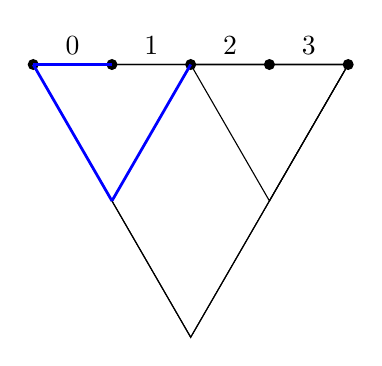
\begin{tikzpicture}
    \coordinate (A) at (0, 0);
    \coordinate (B) at (4, 0);
    \coordinate (C) at (2.0, -3.4641016151377544);
    
    \draw (A) -- (B) -- (C) -- cycle;
    
    \foreach \i in {0,1,...,3} { 
        \draw (\i, 0) -- (\i+1, 0);
    }
    
    \foreach \i in {0,1,...,4} { 
        \fill (\i, 0) circle (2pt);
    }
    
    \foreach \i in {0,1,...,3} { 
        \node[above] at ($ (\i+0.5, 0) $) {\i};
    }
    
    \coordinate (P0) at (0, 0);
    \coordinate (P1) at (2, 0);
    \coordinate (P2) at (1.0, -1.7320508075688772);
    
    \coordinate (P3) at (2, 0);
    \coordinate (P4) at (4, 0);
    \coordinate (P5) at (3.0, -1.7320508075688772);
    \draw (P3) -- (P4) -- (P5) -- cycle;
    
    \coordinate (P6) at (0, 0);
    \coordinate (P7) at (4, 0);
    \coordinate (P8) at (2.0, -3.4641016151377544);
    \draw (P6) -- (P7) -- (P8) -- cycle;

    \draw[blue, line width=1pt] (0,0) -- (1,0);
    \draw[blue, line width=1pt] (P0) -- (P2);
    \draw[blue, line width=1pt] (P1) -- (P2);
  \end{tikzpicture}
  \caption{Visual representation of the protocol $(d0, s0, d1, s2, s1)$. A triangle joining two segments represents entanglement swapping between adjacent links. The blue lines represent the distillations.}
  \label{fig:triangle_notation}
\end{figure}

Considering a protocol with $N$ nodes and $S=N-1$ segments, restrictions implied by this notation are:
\begin{enumerate}
  \item a protocol must perform exactly $S$ entanglement swapping operations,
  \item $d\{i\}$ is allowed only if $s\{i\}$ has not been performed yet, otherwise the protocol is invalid.
\end{enumerate}

For example, $(d0, s0, \textcolor{red}{d0}, s2, s1)$ is not valid, as the joined segment 0-1 is represented by $s1$ after entanglement swapping has been performed to join the two segments, and so $\textcolor{red}{d0}$ does not have any meaning.

\section*{Size of the Protocol Space}

The size of the protocol space is given by the number of possible sequences of swaps and distillations, considering the restrictions imposed by the notation. The number of valid possible sequences of swaps is given by the number of Catalan numbers of $N-2$.
\\\\
When considering distillations, we define $\kappa$ as the maximum number of distillations allowed by a segment ${{i}}$, and we iterate over all possible values of $\kappa$ from 0 to a maximum number of distillations per segment $\beta$.
\footnotetext[1]{From numerical results, I just searched the series here \url{https://oeis.org/search?q=1,5,40,385&language=english&go=Search}.}
Thus, considering $N$ nodes, $S$ segments, and $\kappa$ distillations per segment, the number of possible repeater protocols is given by the Generalized Catalan number \footnotemark[1] of order $S$ and parameter $\kappa+1$, over all $\kappa$ from 0 to $\beta$:
\begin{equation}
    |P| = \sum_{\kappa=0}^{\beta} C(S, \kappa+1) ,
\end{equation}
where:
\begin{equation}
    C(n,k)= \binom{(k+1)*n-2}{n} \cdot \frac{1}{(k*n-1)} .
\end{equation}

\section*{Methodology}

\subsection*{Encoding for Bayesian optimization}

We encode a protocol by starting from two real values $\gamma$ and $\zeta$:
\begin{itemize}
    \item \(\gamma\) represents the symmetricity of the protocol,
    \item \(\zeta\): represents the centering of the rounds of distillation,
\end{itemize}
they are both arbitrary real values between $0$ and $1$.
\\\\
Considering a protocol with $N=2^n+1$ for an integer $n$, the most symmetric protocol (yielded by \(\gamma=1\)), corresponds to the protocol which can be run by Boxi Li machinery.
For example, for $N=5$, the most symmetric protocol $(s0, s2, s1)$ corresponds to the protocol $(0,0)$.
All the non-symmetric protocols considered cannot be represented in the Boxi Li machinery.
\\\\
The encoding returns a tuple which represents the sequence of swaps and rounds of distillation to be performed.
\\\\
The protocol is generated as follows:
\begin{enumerate}
    \item The set of all possible sequences of swaps $P_{swap}$ is generated. 
    They are ordered by the symmetricity of the shape of the swaps, from the least symmetric to the most symmetric. The \((\gamma \times |P_{swap}|\)) sequence is selected, so that:
    \begin{itemize}
        \item if \(\gamma = 0\), the least symmetric sequence is selected,
        \item if \(\gamma = 1\), the most symmetric sequence is selected.
    \end{itemize}
    \item For the selected sequence of swaps, the set of all possible sequences of distillations is generated:
    \[
    \text{seq} = (D_0, \text{swap}_0, D_1, \text{swap}_1, D_2, \ldots, D_S, \text{swap}_{S-1}, D_S)
    \]
    where \(D_0, D_1, \ldots, D_S\) are the sequences of distillations. 
    A sequence $D_i$ is generated by considering the swaps performed so far, can include from $0$ to up to a maximum rounds of distillation per segment per level.
    We consider all the possible joined sequences of swaps and distillations $P_{joined}$, ordered from the lowest to the highest  number of rounds of distillations performed. 
    The \((\zeta \times |P_{joined}|)\) sequence is selected, such that:
    \begin{itemize}
        \item if \(\zeta = 0\), the sequence with no rounds of distillation is selected.
        \item if \(\zeta = 1\), the sequence with the maximum number of rounds of distillation is selected.
    \end{itemize}
\end{enumerate}

\clearpage
\section*{Validation (old protocol space results)}

\begin{table}[ht!]
  \centering
  \begin{tabular}{|c|c|c|c|c|}
      \hline
      BF time & BF Results & GP time & GP result & $|P|$ \\
      \hline
      2155m42.742s & $0.76 \times 10^{-4}$ & 114m23.912s & $0.76 \times 10^{-4}$ & $5.12 \times 10^{3}$ \\
      & *\footnotemark[1] & & *\footnotemark[1] & \\
      \hline
  \end{tabular}
  \caption{Bruteforce of all the \textbf{asymmetric protocols} for $N=5$ and up to 1 round of distillation per segment per level, and corresponding Bayesian optimization. The parameter regime is $p_{gen} = 9.2 \times 10^{-4}$, $w_0 = 0.952$, $t_{coh} = 1.4 \times 10^6$, equivalent to Case C of Table \ref{tab:hardware_regimes}. \\ Bayesian optimizations are performed with 20 initial points and a total of 200 shots.}
  \label{tab:validation_regimes}
\end{table}
\footnotetext[1]{('d0', 'd1', 'd2', 'd3', 's0', 'd2', 'd3', 's2', 'd1', 's1')}


\begin{figure}[ht!]
  \centering
  \includegraphics[width=\linewidth, trim=10 10 10 20, clip]{asymmetric/old_protocol_space/results_gp_tcoh1400000_pgen0.00092_pswap0.85_w00.9524_nodes5_maxdists1/0.9524_2_swaps_skopt_gp.png}
  \caption{Results of the GP optimization for 5 nodes, and max distance 1. The algorithm converges to the optimal protocol in less than 200 evaluations, while a bruteforce algorithm must evaluate all the 5120 protocols.}
  \label{fig:gp_results}
\end{figure}

\clearpage
\section*{Results (old protocol space results)}

\begin{table}[ht!]
    \centering
    \begin{tabular}{|c|c|c|c|c|c|}
        \hline
        Description & $L_0$ (km) & $t_{\text{coh}}^*$ & $w_0 (F_0)$ & $p_{gen}$ \\
        \hline
        \hline
        A: Baseline value, 2 nodes & 200  & $3.6 \times 10^5$ & 0.36 (0.52) & $9.6 \times 10^{-8}$ \\
        \hline
        B: Baseline value, 3 nodes & 100  & $7.2 \times 10^5$ & 0.867 (0.9) & $1.5 \times 10^{-5}$ \\
        \hline
        C: The Hague - Leiden, 5 nodes & 50  & $1.4 \times 10^6$ & 0.952 (0.964) & $9.2 \times 10^{-4}$ \\
        \hline
        D: Delft - The Hague, 10 nodes & 20  & $3.6 \times 10^6$ & 0.958 (0.968) & $2.6 \times 10^{-3}$ \\
        \hline
    \end{tabular}
    \caption{\textbf{Hardware Regimes}. \quad **20min = 2600s}
    \label{tab:hardware_regimes}
\end{table}

\begin{table}[ht!]
    \centering
    \begin{tabular}{|c|c|c|c|c|c|}
        \hline
        & BF time & BF Results & GP time & GP result & $|P|$ \\
        \hline
        \hline
        A & / & / & / & / & 6 \\
        \hline
        B & 152m23.670s & 0.0 & 19min & 0.0 & 21 \\
        & & (no best) & & (no best) & \\
        \hline
        C & 17min & $0.79 \times 10^{-4}$ & 6min & $0.79 \times 10^{-4}$ & 56 \\
        & & (1,1,0,0) & & $(1,1,0,0)$ & \\
        \hline
    \end{tabular}
    \caption{\textbf{Symmetric Protocols}, from 0 to 5 rounds of distillation. All the simulations have been run on the Deigo cluster. Bayesian optimizations are performed with 2 initial points and a total of 20 shots.}
    \label{tab:symmetric_protocols}
\end{table}

\begin{table}[ht!]
    \centering
    \begin{tabular}{|c|c|c|c|c|c|}
        \hline
        & BF time & BF Results & GP time & GP result & $|P|$ \\
        \hline
        \hline
        A & / & / & / & / & 3 \\
        \hline
        B & 83m32.117s & 0.0 & / & / & 27 \\
          & & (no best) & & & \\
        \hline
        C & unfeasible* & / & 144m & $7.5 \times 10^{-5}$ & $2.9 \times 10^{5}$ \\
          & & & *\footnotemark[2] & & \\
        \hline
        D & unfeasible** & / & ... & ... & $4.2 \times 10^{24}$ \\
          & & & & & \\
        \hline
    \end{tabular}
    \caption{\textbf{Asymmetric Protocols}, up to 1 round of distillation per segment per level. 
    Bayesian optimizations are performed with 20 initial points and a total of 200 shots. \\ * for 1 round of dist, we have the case presented in Table \ref{tab:validation_regimes} ($|P| = 5120$), but for higher rounds, the optimization is unfeasible. \\ ** for 0 rounds of dist, $|P| = 1430$ and $skr=0.0$ in (1420m50.592s), but for higher rounds, the optimization is unfeasible.}
    \label{tab:asymmetric_protocols}
\end{table}

\footnotetext[2]{('d1', 'd1', 'd2', 'd3', 's1', 'd0', 'd0', 'd3', 's2', 'd0', 's0')}

We present Case C of Table \ref{tab:symmetric_protocols} in Figure \ref{fig:symmetric_5_nodes}. We also present Case C of Table \ref{tab:asymmetric_protocols} in Figure \ref{fig:asymmetric_5_nodes}.

\begin{figure}[ht!]
  \centering
  \includegraphics[width=\linewidth]{symmetric/results_gp_centerspace/0.9524_2_swaps_skopt_gp.png}  
  \caption{Results of the GP optimization for 5 nodes (2 symmetric swaps), and up to 5 rounds of distillation (applied to all links in the level). The algorithm converges to the optimal protocol in less than 20 evaluations, while a bruteforce algorithm must evaluate 56 protocols.}
  \label{fig:symmetric_5_nodes}
\end{figure}

\begin{figure}[ht!]
  \centering
  \includegraphics[width=\linewidth]{asymmetric/old_protocol_space/results_gp_tcoh1400000_pgen0.00092_pswap0.85_w00.952_nodes5_maxdists2/skopt_gp.png}
  \caption{Results of the GP optimization for 5 nodes (asymmetric), and up to 2 rounds of distillation. The algorithm converges to the maximum in around $100$ evaluations, out of the $295245$. However, we know that this is a sub-optimal result, as a higher secret key rate is yielded by the symmetric protocol presented in \ref{fig:symmetric_5_nodes}.}
  \label{fig:asymmetric_5_nodes}
\end{figure}

\end{document}



\end{document}
